\documentclass{standalone}
\usepackage{tikz}
\usetikzlibrary{patterns, positioning}
\usepackage[sfdefault]{ClearSans} %% option 'sfdefault' activates Clear Sans as the default text font
\usepackage[T1]{fontenc}

\begin{document}
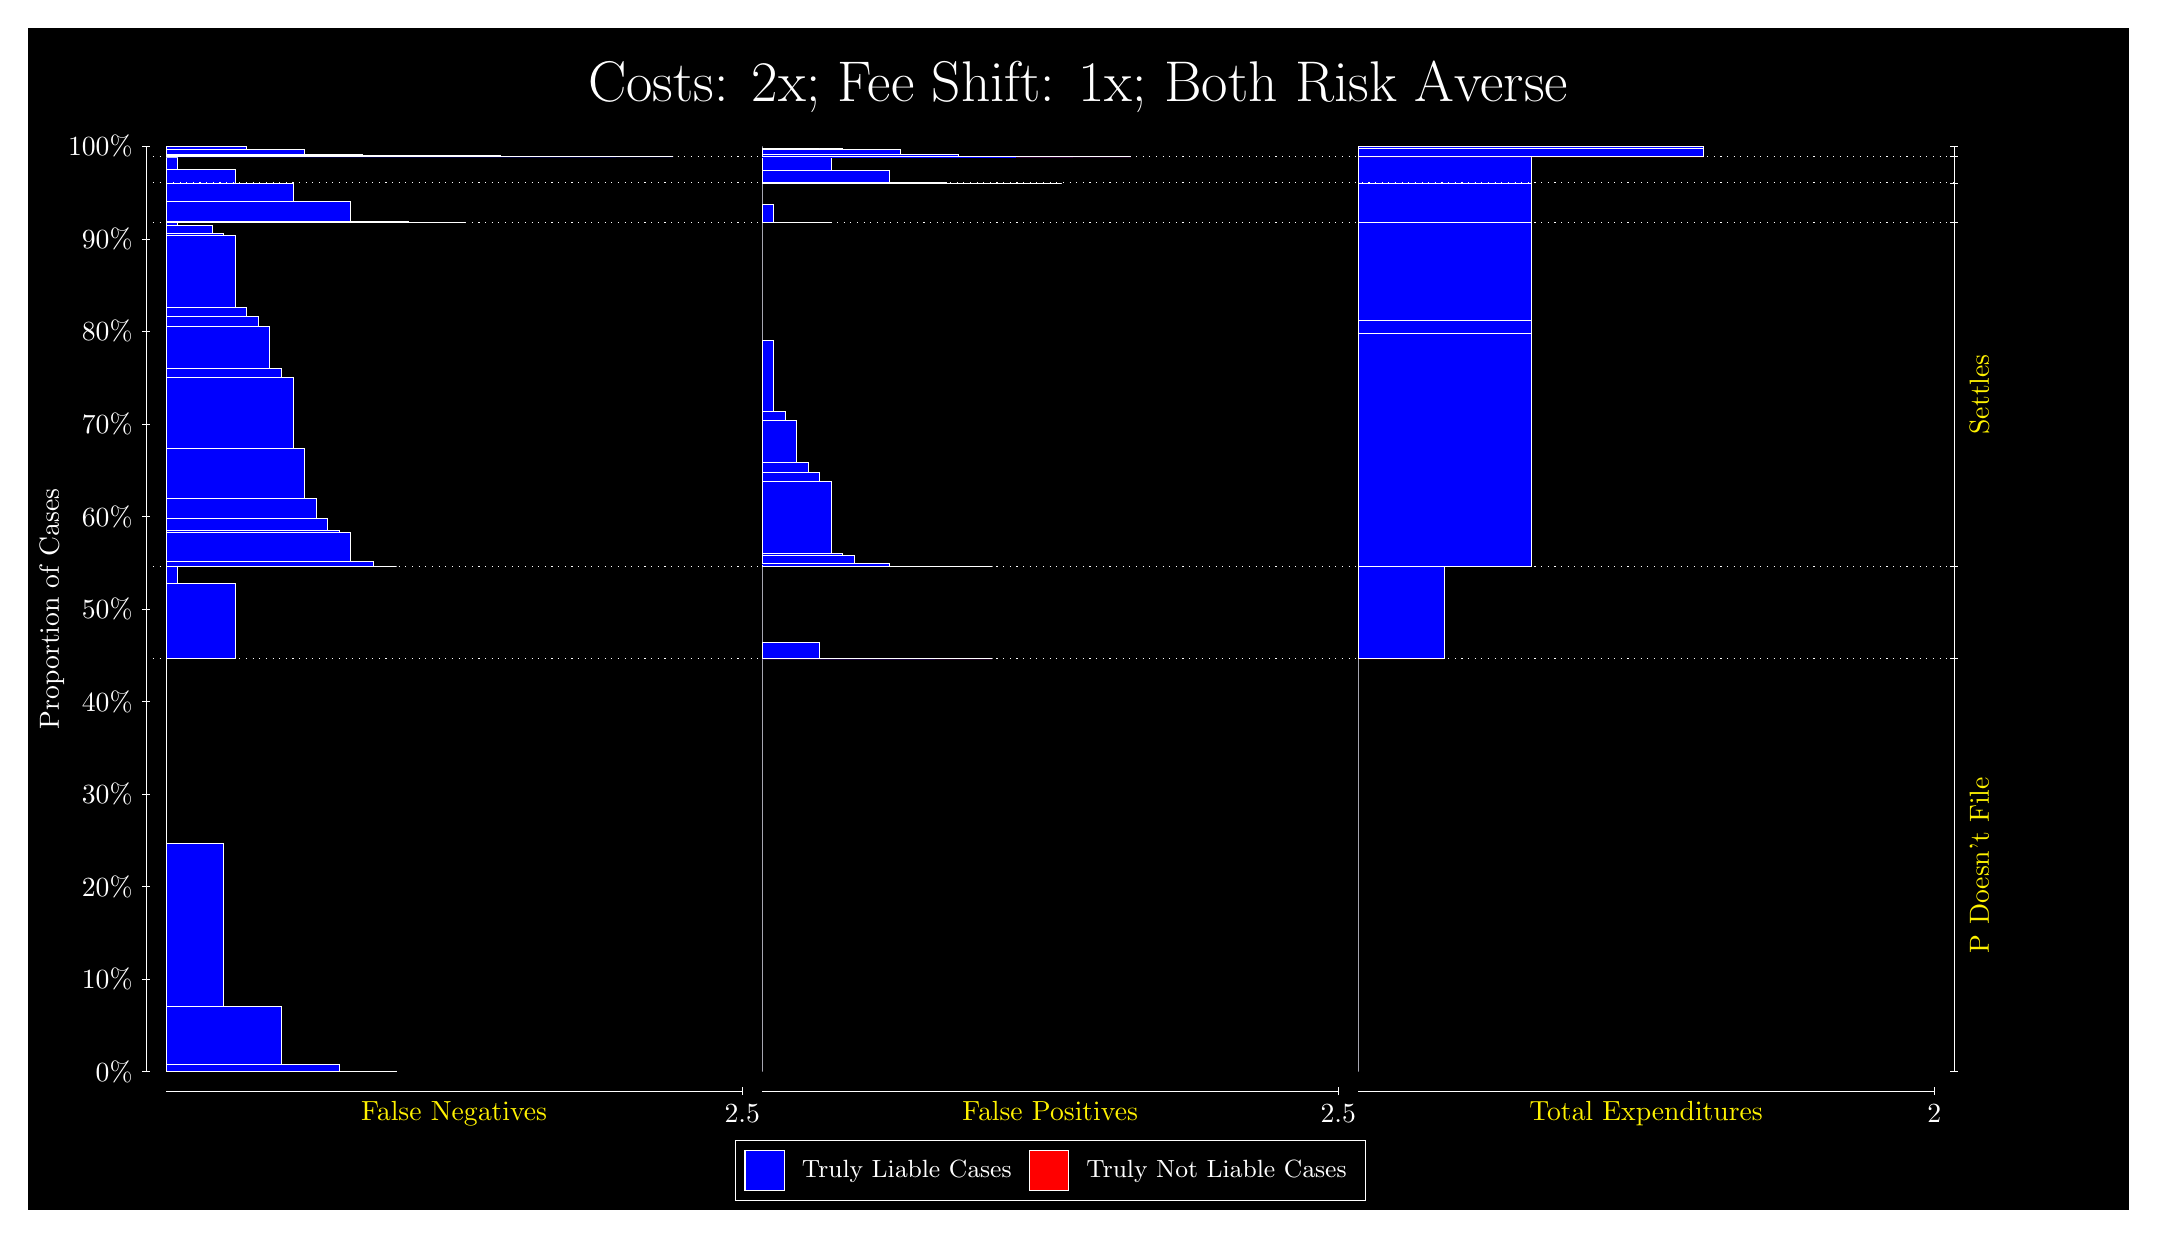
\begin{tikzpicture}
\draw[fill=black] (0,0) rectangle (26.667,15);
\draw[text=white] (0,13.5) rectangle (26.667,15) node[midway] {\huge Costs: 2x; Fee Shift: 1x; Both Risk Averse};
\draw[white, very thin] (1.5,1.75) -- (1.5,13.5);
\node[rotate=90, text=white, anchor=center] at (0.3, 7.625) {Proportion of Cases};
\draw[white, very thin] (1.45,1.75) -- (1.55,1.75);
\node[text=white, anchor=east] at (1.45, 1.75) {0\%};
\draw[white, very thin] (1.45,2.925) -- (1.55,2.925);
\node[text=white, anchor=east] at (1.45, 2.925) {10\%};
\draw[white, very thin] (1.45,4.1) -- (1.55,4.1);
\node[text=white, anchor=east] at (1.45, 4.1) {20\%};
\draw[white, very thin] (1.45,5.275) -- (1.55,5.275);
\node[text=white, anchor=east] at (1.45, 5.275) {30\%};
\draw[white, very thin] (1.45,6.45) -- (1.55,6.45);
\node[text=white, anchor=east] at (1.45, 6.45) {40\%};
\draw[white, very thin] (1.45,7.625) -- (1.55,7.625);
\node[text=white, anchor=east] at (1.45, 7.625) {50\%};
\draw[white, very thin] (1.45,8.8) -- (1.55,8.8);
\node[text=white, anchor=east] at (1.45, 8.8) {60\%};
\draw[white, very thin] (1.45,9.975) -- (1.55,9.975);
\node[text=white, anchor=east] at (1.45, 9.975) {70\%};
\draw[white, very thin] (1.45,11.15) -- (1.55,11.15);
\node[text=white, anchor=east] at (1.45, 11.15) {80\%};
\draw[white, very thin] (1.45,12.325) -- (1.55,12.325);
\node[text=white, anchor=east] at (1.45, 12.325) {90\%};
\draw[white, very thin] (1.45,13.5) -- (1.55,13.5);
\node[text=white, anchor=east] at (1.45, 13.5) {100\%};

\draw[white, very thin] (24.457,1.75) -- (24.457,13.5);
\draw[white, very thin] (24.407,1.75) -- (24.507,1.75);
\node[anchor=west] at (24.407, 1.75) {};
\draw[white, very thin] (24.407,6.9929) -- (24.507,6.9929);
\node[anchor=west] at (24.407, 6.9929) {};
\draw[white, very thin] (24.407,8.1672) -- (24.507,8.1672);
\node[anchor=west] at (24.407, 8.1672) {};
\draw[white, very thin] (24.407,12.534) -- (24.507,12.534);
\node[anchor=west] at (24.407, 12.534) {};
\draw[white, very thin] (24.407,13.036) -- (24.507,13.036);
\node[anchor=west] at (24.407, 13.036) {};
\draw[white, very thin] (24.407,13.369) -- (24.507,13.369);
\node[anchor=west] at (24.407, 13.369) {};
\draw[white, very thin] (24.407,13.5) -- (24.507,13.5);
\node[anchor=west] at (24.407, 13.5) {};

\draw[white, very thin, fill=blue] (1.75,1.75) rectangle (4.6775,1.7509);
\draw[white, very thin, fill=blue] (1.75,1.7509) rectangle (3.9457,1.8397);
\draw[white, very thin, fill=blue] (1.75,1.8397) rectangle (3.2138,2.5836);
\draw[white, very thin, fill=blue] (1.75,2.5836) rectangle (2.4819,4.6458);
\draw[white, very thin, fill=red] (1.75,4.6458) rectangle (1.75,4.6458);
\draw[white, very thin, fill=blue] (1.75,4.6458) rectangle (1.75,6.9929);
\draw[white, very thin, fill=blue] (1.75,6.9929) rectangle (2.6283,7.9546);
\draw[white, very thin, fill=blue] (1.75,7.9546) rectangle (1.8964,8.1614);
\draw[white, very thin, fill=red] (1.75,8.1614) rectangle (1.75,8.1614);
\draw[white, very thin, fill=blue] (1.75,8.1614) rectangle (1.75,8.1672);
\draw[white, very thin, fill=blue] (1.75,8.1672) rectangle (4.6775,8.1672);
\draw[white, very thin, fill=blue] (1.75,8.1672) rectangle (4.3848,8.2349);
\draw[white, very thin, fill=blue] (1.75,8.2349) rectangle (4.092,8.5977);
\draw[white, very thin, fill=blue] (1.75,8.5977) rectangle (3.9457,8.6264);
\draw[white, very thin, fill=blue] (1.75,8.6264) rectangle (3.7993,8.7709);
\draw[white, very thin, fill=blue] (1.75,8.7709) rectangle (3.6529,9.029);
\draw[white, very thin, fill=blue] (1.75,9.029) rectangle (3.5065,9.6665);
\draw[white, very thin, fill=blue] (1.75,9.6665) rectangle (3.3602,10.561);
\draw[white, very thin, fill=blue] (1.75,10.561) rectangle (3.2138,10.675);
\draw[white, very thin, fill=blue] (1.75,10.675) rectangle (3.0674,11.213);
\draw[white, very thin, fill=blue] (1.75,11.213) rectangle (2.921,11.347);
\draw[white, very thin, fill=blue] (1.75,11.347) rectangle (2.7746,11.459);
\draw[white, very thin, fill=blue] (1.75,11.459) rectangle (2.6283,12.375);
\draw[white, very thin, fill=blue] (1.75,12.375) rectangle (2.4819,12.397);
\draw[white, very thin, fill=blue] (1.75,12.397) rectangle (2.3355,12.495);
\draw[white, very thin, fill=blue] (1.75,12.495) rectangle (2.1891,12.5);
\draw[white, very thin, fill=blue] (1.75,12.5) rectangle (2.0428,12.5);
\draw[white, very thin, fill=blue] (1.75,12.5) rectangle (1.8964,12.534);
\draw[white, very thin, fill=red] (1.75,12.534) rectangle (1.75,12.534);
\draw[white, very thin, fill=blue] (1.75,12.534) rectangle (1.75,12.534);
\draw[white, very thin, fill=blue] (1.75,12.534) rectangle (5.5558,12.534);
\draw[white, very thin, fill=blue] (1.75,12.534) rectangle (4.8239,12.543);
\draw[white, very thin, fill=blue] (1.75,12.543) rectangle (4.092,12.808);
\draw[white, very thin, fill=blue] (1.75,12.808) rectangle (3.3602,13.033);
\draw[white, very thin, fill=blue] (1.75,13.033) rectangle (2.6283,13.036);
\draw[white, very thin, fill=red] (1.75,13.036) rectangle (1.75,13.036);
\draw[white, very thin, fill=blue] (1.75,13.036) rectangle (2.6283,13.209);
\draw[white, very thin, fill=blue] (1.75,13.209) rectangle (1.8964,13.365);
\draw[white, very thin, fill=red] (1.75,13.365) rectangle (1.75,13.365);
\draw[white, very thin, fill=blue] (1.75,13.365) rectangle (1.75,13.369);
\draw[white, very thin, fill=blue] (1.75,13.369) rectangle (8.1906,13.369);
\draw[white, very thin, fill=blue] (1.75,13.369) rectangle (7.4587,13.369);
\draw[white, very thin, fill=blue] (1.75,13.369) rectangle (6.7268,13.372);
\draw[white, very thin, fill=blue] (1.75,13.372) rectangle (5.9949,13.386);
\draw[white, very thin, fill=blue] (1.75,13.386) rectangle (5.7022,13.386);
\draw[white, very thin, fill=blue] (1.75,13.386) rectangle (5.2631,13.387);
\draw[white, very thin, fill=blue] (1.75,13.387) rectangle (4.9703,13.388);
\draw[white, very thin, fill=blue] (1.75,13.388) rectangle (4.5312,13.388);
\draw[white, very thin, fill=blue] (1.75,13.388) rectangle (4.2384,13.404);
\draw[white, very thin, fill=blue] (1.75,13.404) rectangle (3.7993,13.404);
\draw[white, very thin, fill=blue] (1.75,13.404) rectangle (3.5065,13.468);
\draw[white, very thin, fill=blue] (1.75,13.468) rectangle (2.7746,13.498);
\draw[white, very thin, fill=blue] (1.75,13.498) rectangle (2.0428,13.5);
\draw[white, very thin, fill=red] (1.75,13.5) rectangle (1.75,13.5);
\draw[white, very thin, fill=blue] (1.75,13.5) rectangle (1.75,13.5);
\draw[white, very thin, fill=red] (9.3189,1.75) rectangle (9.3189,1.75);
\draw[white, very thin, fill=blue] (9.3189,1.75) rectangle (9.3189,6.9929);
\draw[white, very thin, fill=red] (9.3189,6.9929) rectangle (12.246,6.9929);
\draw[white, very thin, fill=blue] (9.3189,6.9929) rectangle (12.246,6.9929);
\draw[white, very thin, fill=blue] (9.3189,6.9929) rectangle (11.515,6.9929);
\draw[white, very thin, fill=blue] (9.3189,6.9929) rectangle (10.783,6.9987);
\draw[white, very thin, fill=blue] (9.3189,6.9987) rectangle (10.051,7.2055);
\draw[white, very thin, fill=blue] (9.3189,7.2055) rectangle (9.3189,8.1672);
\draw[white, very thin, fill=red] (9.3189,8.1672) rectangle (12.246,8.1672);
\draw[white, very thin, fill=blue] (9.3189,8.1672) rectangle (12.246,8.1672);
\draw[white, very thin, fill=red] (9.3189,8.1672) rectangle (11.954,8.1672);
\draw[white, very thin, fill=blue] (9.3189,8.1672) rectangle (11.954,8.1672);
\draw[white, very thin, fill=red] (9.3189,8.1672) rectangle (11.661,8.1672);
\draw[white, very thin, fill=blue] (9.3189,8.1672) rectangle (11.661,8.1672);
\draw[white, very thin, fill=blue] (9.3189,8.1672) rectangle (11.515,8.1672);
\draw[white, very thin, fill=red] (9.3189,8.1672) rectangle (11.368,8.1672);
\draw[white, very thin, fill=blue] (9.3189,8.1672) rectangle (11.368,8.1672);
\draw[white, very thin, fill=blue] (9.3189,8.1672) rectangle (11.222,8.1673);
\draw[white, very thin, fill=red] (9.3189,8.1673) rectangle (11.075,8.1673);
\draw[white, very thin, fill=blue] (9.3189,8.1673) rectangle (11.075,8.1674);
\draw[white, very thin, fill=blue] (9.3189,8.1674) rectangle (10.929,8.2008);
\draw[white, very thin, fill=blue] (9.3189,8.2008) rectangle (10.783,8.2014);
\draw[white, very thin, fill=blue] (9.3189,8.2014) rectangle (10.636,8.2059);
\draw[white, very thin, fill=blue] (9.3189,8.2059) rectangle (10.49,8.3038);
\draw[white, very thin, fill=blue] (9.3189,8.3038) rectangle (10.344,8.3257);
\draw[white, very thin, fill=blue] (9.3189,8.3257) rectangle (10.197,9.2416);
\draw[white, very thin, fill=blue] (9.3189,9.2416) rectangle (10.051,9.3544);
\draw[white, very thin, fill=blue] (9.3189,9.3544) rectangle (9.9044,9.4883);
\draw[white, very thin, fill=blue] (9.3189,9.4883) rectangle (9.758,10.026);
\draw[white, very thin, fill=blue] (9.3189,10.026) rectangle (9.6116,10.14);
\draw[white, very thin, fill=blue] (9.3189,10.14) rectangle (9.4652,11.034);
\draw[white, very thin, fill=blue] (9.3189,11.034) rectangle (9.3189,12.534);
\draw[white, very thin, fill=red] (9.3189,12.534) rectangle (10.197,12.534);
\draw[white, very thin, fill=blue] (9.3189,12.534) rectangle (10.197,12.537);
\draw[white, very thin, fill=blue] (9.3189,12.537) rectangle (9.4652,12.762);
\draw[white, very thin, fill=blue] (9.3189,12.762) rectangle (9.3189,13.036);
\draw[white, very thin, fill=red] (9.3189,13.036) rectangle (13.125,13.036);
\draw[white, very thin, fill=blue] (9.3189,13.036) rectangle (13.125,13.036);
\draw[white, very thin, fill=blue] (9.3189,13.036) rectangle (12.393,13.036);
\draw[white, very thin, fill=blue] (9.3189,13.036) rectangle (11.661,13.04);
\draw[white, very thin, fill=blue] (9.3189,13.04) rectangle (10.929,13.196);
\draw[white, very thin, fill=blue] (9.3189,13.196) rectangle (10.197,13.369);
\draw[white, very thin, fill=red] (9.3189,13.369) rectangle (14.003,13.369);
\draw[white, very thin, fill=blue] (9.3189,13.369) rectangle (14.003,13.369);
\draw[white, very thin, fill=red] (9.3189,13.369) rectangle (13.271,13.369);
\draw[white, very thin, fill=blue] (9.3189,13.369) rectangle (13.271,13.369);
\draw[white, very thin, fill=red] (9.3189,13.369) rectangle (12.539,13.369);
\draw[white, very thin, fill=blue] (9.3189,13.369) rectangle (12.539,13.37);
\draw[white, very thin, fill=blue] (9.3189,13.37) rectangle (11.807,13.4);
\draw[white, very thin, fill=red] (9.3189,13.4) rectangle (11.807,13.4);
\draw[white, very thin, fill=blue] (9.3189,13.4) rectangle (11.807,13.4);
\draw[white, very thin, fill=blue] (9.3189,13.4) rectangle (11.075,13.464);
\draw[white, very thin, fill=blue] (9.3189,13.464) rectangle (11.075,13.465);
\draw[white, very thin, fill=red] (9.3189,13.465) rectangle (10.783,13.465);
\draw[white, very thin, fill=blue] (9.3189,13.465) rectangle (10.783,13.465);
\draw[white, very thin, fill=blue] (9.3189,13.465) rectangle (10.344,13.473);
\draw[white, very thin, fill=blue] (9.3189,13.473) rectangle (10.344,13.481);
\draw[white, very thin, fill=red] (9.3189,13.481) rectangle (10.051,13.481);
\draw[white, very thin, fill=blue] (9.3189,13.481) rectangle (10.051,13.481);
\draw[white, very thin, fill=blue] (9.3189,13.481) rectangle (9.6116,13.481);
\draw[white, very thin, fill=blue] (9.3189,13.481) rectangle (9.6116,13.481);
\draw[white, very thin, fill=red] (9.3189,13.481) rectangle (9.3189,13.481);
\draw[white, very thin, fill=blue] (9.3189,13.481) rectangle (9.3189,13.5);
\draw[white, very thin, fill=red] (16.888,1.75) rectangle (16.888,1.75);
\draw[white, very thin, fill=blue] (16.888,1.75) rectangle (16.888,6.9929);
\draw[white, very thin, fill=red] (16.888,6.9929) rectangle (17.986,6.9929);
\draw[white, very thin, fill=blue] (16.888,6.9929) rectangle (17.986,8.1672);
\draw[white, very thin, fill=red] (16.888,8.1672) rectangle (19.083,8.1672);
\draw[white, very thin, fill=blue] (16.888,8.1672) rectangle (19.083,11.124);
\draw[white, very thin, fill=red] (16.888,11.124) rectangle (19.083,11.124);
\draw[white, very thin, fill=blue] (16.888,11.124) rectangle (19.083,11.289);
\draw[white, very thin, fill=red] (16.888,11.289) rectangle (19.083,11.289);
\draw[white, very thin, fill=blue] (16.888,11.289) rectangle (19.083,12.534);
\draw[white, very thin, fill=red] (16.888,12.534) rectangle (19.083,12.534);
\draw[white, very thin, fill=blue] (16.888,12.534) rectangle (19.083,13.036);
\draw[white, very thin, fill=red] (16.888,13.036) rectangle (19.083,13.036);
\draw[white, very thin, fill=blue] (16.888,13.036) rectangle (19.083,13.369);
\draw[white, very thin, fill=red] (16.888,13.369) rectangle (21.279,13.369);
\draw[white, very thin, fill=blue] (16.888,13.369) rectangle (21.279,13.473);
\draw[white, very thin, fill=red] (16.888,13.473) rectangle (21.279,13.473);
\draw[white, very thin, fill=blue] (16.888,13.473) rectangle (21.279,13.5);
\draw[white, dotted] (1.5,6.9929) -- (24.457,6.9929);
\draw[white, dotted] (1.5,8.1672) -- (24.457,8.1672);
\draw[white, dotted] (1.5,12.534) -- (24.457,12.534);
\draw[white, dotted] (1.5,13.036) -- (24.457,13.036);
\draw[white, dotted] (1.5,13.369) -- (24.457,13.369);
\draw[white, very thin] (1.75,1.5) -- (9.0689,1.5);
\node[text=yellow, anchor=north] at (5.4094, 1.5) {False Negatives};
\draw[white, very thin] (9.0689,1.45) -- (9.0689,1.55);
\node[text=white, anchor=north] at (9.0689, 1.45) {2.5};

\draw[white, very thin] (9.3189,1.5) -- (16.638,1.5);
\node[text=yellow, anchor=north] at (12.978, 1.5) {False Positives};
\draw[white, very thin] (16.638,1.45) -- (16.638,1.55);
\node[text=white, anchor=north] at (16.638, 1.45) {2.5};

\draw[white, very thin] (16.888,1.5) -- (24.207,1.5);
\node[text=yellow, anchor=north] at (20.547, 1.5) {Total Expenditures};
\draw[white, very thin] (24.207,1.45) -- (24.207,1.55);
\node[text=white, anchor=north] at (24.207, 1.45) {2};

\node[text=yellow, centered, rotate=90] at (24.777, 4.3715) {P Doesn't File};

\node[text=yellow, centered, rotate=90] at (24.777, 10.35) {Settles};




\draw (12.978300999999998,1.5) node[draw=none] (baseCoordinate) {};
\begin{scope}[align=center]
        \matrix[scale=0.5, draw=white, below=0.5cm of baseCoordinate, nodes={draw}, column sep=0.1cm]{
            \node[rectangle, draw, minimum width=0.5cm, minimum height=0.5cm, fill=blue] {}; &
            \node[draw=none, font=\small, text=white] (B) {Truly Liable Cases}; &
            \node[rectangle, draw, minimum width=0.5cm, minimum height=0.5cm, fill=red] {}; &
            \node[draw=none, font=\small, text=white] (B) {Truly Not Liable Cases}; \\
            };
\end{scope}

\end{tikzpicture}
\end{document}